\begin{figure*}[b]
	\centering
	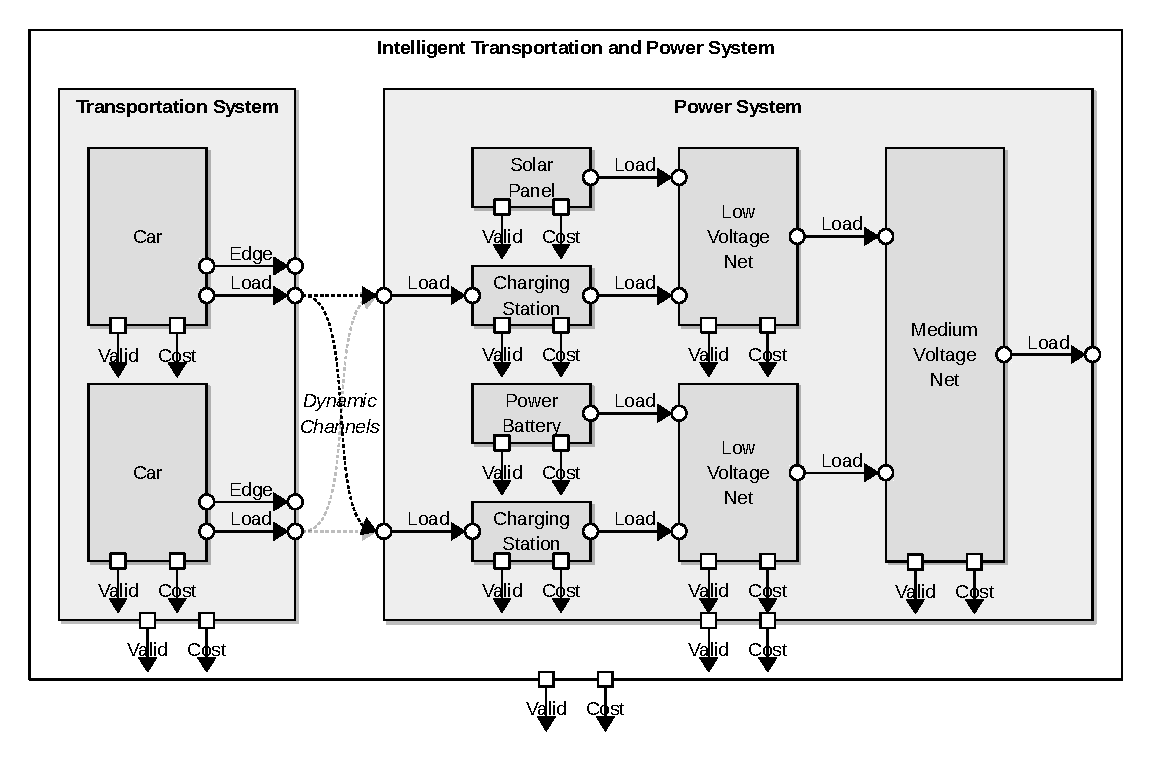
\includegraphics[width=\textwidth]{../gfx/model.pdf}
	\caption{Overview of the holistic modeling approach including transportation and power system connected by dynamic channels.}
	\label{fig:model}
\end{figure*}

\section{Transportation and power system modeling}
\label{section:contribution}

Based on the underlying systems modeling technique, we now propose an integrated transportation and power system model as shown in Figure~\ref{fig:model}. At its root, the model defines an intelligent transportation and power system component, which contains separate components for the transportation and the power system. The transportation system component comprises the individual car components traveling along the traffic infrastructure. Similarly, the power system component includes the individual electric components, such as static loads, solar panels, power batteries and charging stations. Furthermore, the power system component contains the electric infrastructure consisting of low-voltage and medium-voltage net components. Parametrization allows one to instantiate all components using reference configurations, i.e. predefined parameter valuations. Subsequently we describe the different components of the model in terms of their parameters, ports, channels and behavior. Furthermore, for each parameter we provide a description as well as a reference configuration.

\subsection{Intelligent transportation and power system}

The intelligent transportation and power system $IS$ is a structure which contains the transportation and the power system. It encodes dynamic channels between the output car loads of the transportation system and the input car loads of the power system. The output car loads of the transportation represent the source ports, while respective car positions of the transportation system represent source port options in each port/option pair. In return, input car loads of the power system and charging station positions of the power system are registered to the respective dynamic channels. 

\begin{table}[h]
	\renewcommand{\arraystretch}{1.3}
	%\caption{Intelligent transportation and power system parameters}
	\centering
	\begin{tabularx}{\columnwidth}{lllllX}
		\hline
		\textbf{Parameter}      & \textbf{$IS_{A}$} & \textbf{$IS_{B}$}  & \textbf{$IS_{C}$} & \textbf{$IS_{D}$}      & \textbf{Description} \\ \hline
		TN               & $...$ 	& $...$ & $...$ & $...$ 	  	& Traffic network (Graph)     					\\
		TS     					& $TS_{A}$   	& $TS_{A}$ & $TS_{A}$ & $TS_{A}$	 	& Transportation system     			\\
		PS               		& $PS_{A}$ 	& $PS_{A}$ & $PS_{B}$ & $PS_{B}$		& Power system   						\\
		w\_TS              & $0.75$  	& $0.25$ & $0.25$ & $0.25$		& Weight of transportation system costs (\%)	\\ 
		w\_PS              & $0.25$  	& $0.75$ & $0.75$ & $0.75$  		& Weight of power system costs (\%)   			\\ \hline
	\end{tabularx}
\end{table}

In terms of behavior, the intelligent transportation and power system specifies a cost function which aggregates the cost of the transportation and the power system using the weight parameters $Weight\_TS$ and $Weight\_PS$. On this cost function a minimization objective is defined.

\subsection{Transportation system}

The transportation system $TS$ is a structure representing the traffic infrastructure with it's cars. Specifically, the transportation system is consisted of cars of different types, modeled as a distribution over multiple car types. The traffic infrastructure is modeled as a directed graph $G = (V,E)$, an ordered pair consisting of a finite set of nodes $V$ and edges $E \subseteq V \times V$, i.e. directed connections between nodes. Here, nodes $V$ represent reference points in the environment such as intersections. Nodes are defined by absolute position based on real-world coordinates, i.e. latitude, longitude, and elevation. Edges $E \subseteq V \times V$ represent road segments between these reference points with source $v$ and target $w$ nodes and $(v,w) \in E$. Furthermore, edges are defined through an assigned number of lanes and a possessed road type, such as residential streets or stations.

\begin{table}[h]
	\renewcommand{\arraystretch}{1.3}
	%\caption{Transportation system parameters}
	\centering
	\begin{tabularx}{\columnwidth}{llX}
		\hline
		\textbf{Parameter}     & \textbf{$TS_{A}$}         & \textbf{Description} \\ \hline
		TN              & $G$    & Traffic network (Graph)    \\
		Car\_Number            & $240$    & Number of cars (\#)      \\ 
		Car\_Frequency      & $\{C_{A},C_{B},C_{C}\}:0.\overline{3}$    & Frequency of different car types (\%)       \\ \hline
	\end{tabularx}
\end{table}

In terms of behavior, the transportation system specifies a cost function which aggregates the costs of the individual car components it contains. For this, the costs of cars are multiplied by the individual priority specified for each car. These costs are aggregated to a single cost function. To ensure valid behavior, the transportation system implements a constraint on the car components which tests if cars overlap on their respective positions on the traffic network.

\subsection{Car}

Cars $C$ represent entities within the transportation system, which are are defined by their position on the traffic network. In terms of physical representation, they are defined through their length and weight. Furthermore, they hold a battery of given capacity, i.e. the state of charge. Furthermore, they encode rates defining the power transfer rate between car battery and charging stations.

\begin{table}[h]
	\renewcommand{\arraystretch}{1.3}
	%\caption{Car parameters}
	\centering
	\begin{tabularx}{\columnwidth}{llllX}
		\hline
		\textbf{Parameter}          & \textbf{$C_{A}$} & \textbf{$C_{B}$}  & \textbf{$C_{C}$}           & \textbf{Description} \\ \hline
		Origin                      & $E$     & $E$ & $E$    & Origin Position (Edge)      \\
		Destination                 & $E$    & $E$  & $E$     & Destination Position (Edge) \\
		Weight\_SOC              & $0.\overline{3}$  & $0.\overline{3}$ & $0.\overline{3}$ & Weight of state of charge costs (\%)                   \\
		Weight\_Time              & $0.\overline{3}$ & $0.\overline{3}$ & $0.\overline{3}$ & Weight of time costs (\%)                     \\
		Weight\_Power             & $0.\overline{3}$ & $0.\overline{3}$ & $0.\overline{3}$ & Weight of power costs (\%)                      \\
		Priority                  & $1.0$ & $1.0$ & $1.0$ & Priority of the car in traffic (\%)                  \\
		Length                    & $4.0$ & $4.0$ & $4.0$ & Car length (Meters)            \\
		Weight                   & $2.0$ & $2.0$ & $2.0$ & Car weight  (Tonnes)                 \\
		SOC                      & $30.0$ & $60.0$ & $90.0$ & Initial state of charge (kW/h)                   \\
		SOC\_Min               & $0.0$ & $0.0$ & $0.0$ & Min. state of charge (kW/h)                     \\
		SOC\_Max              & $90.0$ & $90.0$ & $90.0$ & Max state of charge (kW/h)                      \\
		Charge\_Rate          & $5.0$ & $5.0$ & $5.0$ & Battery (dis-)charge rate (kW/h)                    \\
		Range\_Anxiety         & $0.2$ & $0.2$ & $0.2$ & Affinity to charge (\%)                     \\
		CS\_Selection		   & $0.5$ & $0.5$ & $0.5$ & Charging station randomness (\%)                    \\ 
		Departure\_Time 	& $0$ & $0$ & $0$ & Offset to start traveling (Minutes)                   \\ \hline
	\end{tabularx}
\end{table}

The behavior of cars is described as follows: When the departure time of a car is reached, it begins to travel from origin to destination. Origins, destinations and current position of a car are represented by edges on the traffic network.  When beginning to travel, a car's position is equivalent to the origin, while subsequent positions are selected from a determined route. Specifically, route selection is based on a specified number of alternatives of shortest paths from the current position to the destination or the nearest charging station. Of these alternatives, one route is randomly selected. If the state of charge falls below a specified percentage described by it's range anxiety, the car route selection probability shifts the percentage specified by it's charging station selection randomness. While traveling on the traffic network, cars consume energy based on traveled elevation profile, the car's mass and chosen speed. Within the car, energy consumption or production occurs based on the car's battery from which energy can be subtracted or can be added to. Energy consumption occurs while driving or while discharging the car's battery at a charging station. Energy production occurs through energy recuperation while driving or while charging the car's battery at a charging station. To ensure valid behavior, a constraint tests whether the battery's state of charge lies within a constant minimum and maximum level. When connected to a charging station through a dynamic channel, charging occurs based on a probabilistic selection of states, which are uniformly distributed in terms of their probability. If the car chooses to charge, a defined power load is transferred from the charging station to the car's battery. If the car chooses to discharge, a defined power load (charge rate) is transferred from the car's battery to the charging station. Furthermore, the car can choose a zero state, in which no power load is transferred between car and charging station.

The objectives of a car's behavior are represented through multiple cost functions. Generally, costs of a car can only incur when it's departure time has been reached and are aggregated over time. Firstly, a cost function for the car's convenience measures the cars state of charge in relation to the car's maximum state of charge. Secondly, a cost function for shortest traveling time aggregates the time needed for a car to reach it's destination. Thirdly, a cost function for the car's energy efficiency measures it's energy consumption in relation to the cars maximum energy consumption. The cost functions are aggregated and weighted by the impact of the different objectives by applying specific weights to the given cost functions.

\subsection{Power system}

The power system $PS$ component represents the overall power electric network including each individual electric device as well as the supporting infrastructure (i.e.\ low- and medium-voltage networks).

\begin{table}[h]
	\renewcommand{\arraystretch}{1.3}
	%\caption{Power system parameters}
	\centering
	\begin{tabularx}{\columnwidth}{lllX}
		\hline
		\textbf{Parameter}     & \textbf{$PS_{A}$} & \textbf{$PS_{B}$}       & \textbf{Description} \\ \hline
		TN              & $G$ & $G$    	  & Traffic network (Graph)     \\
		LV\_Number             & $4$ & $4$            & Number of LV (\#)      \\
		LV\_Frequency          & $LV_{A}:1.0$ & $LV_{A}:1.0$                & Freq. of LV types (\%)      \\
		LV\_Allocation         & $9$ & $19$                 & Electric devices per LV (\#)      \\   
		MV\_Number             & $1$ & $1$        & Number of MV (\#)      \\ 
		MV\_Frequency          & $MV_{A}:1.0$ & $MV_{A}:1.0$                & Freq. of MV types (\%)      \\
		MV\_Allocation         & $4$ & $4$                     & LV per MV (\#)      \\   
		SP\_Number             & $5$ & $5$         & Number of SP (\#)      \\ 
		SP\_Frequency          & $SP_{A}:1.0$ & $SP_{B}:1.0$                & Freq. of SP types (\%)       \\  
		CS\_Number             & $16$  & $56$           & Number of CS (\#)      \\
		CS\_Frequency          & $CS_{A}:1.0$  & $CS_{B}:1.0$               & Freq. of CS types (\%)       \\   
		PB\_Number          & $5$  & $5$              & Number of PB (\#)      \\
		PB\_Frequency          & $PB_{A}:1.0$ & $PB_{B}:1.0$              & Freq. of PB types (\%)       \\ 
		SL\_Number          & $10$ & $10$              & Number of SL (\#)      \\
		SL\_Frequency          & $SL_{A}:1.0$ & $SL_{B}:1.0$              & Freq. of SL types (\%)       \\  \hline  
	\end{tabularx}
\end{table}

When looking at its behavior, the power system specifies a cost function that aggregates the costs of contained batteries, solar panels, charging stations as well as low- and medium-voltage networks. In principle, different aggregation schemes can be used. Furthermore, it forwards the load of the medium-voltage network representing the final load balance.

\subsection{Low/medium-voltage networks}

Low- and medium-voltage networks $LV$, $MV$ represent one part of the electric infrastructure. In our model, low- and medium-voltage networks receive the loads of all connected electric devices and provide an aggregate load to the upper voltage level.

\begin{table}[h]
	\renewcommand{\arraystretch}{1.3}
	%\caption{Low/medium voltage net parameters}
	\centering
	\begin{tabularx}{\columnwidth}{lllX}
		\hline
		\textbf{Parameter}   & \textbf{$LV_{A}$} & \textbf{$MV_{A}$}  & Description \\ \hline
		Weight\_Balance       & $0.0$ & $1.0$ & Weight of balance costs (\%) \\  
%		Size                  	  & $9$ & $19$ & Number of devices per net  (\#)    \\
		Capacity          & $20.0$ & $200.0$ & Power load capacity (kW/h)     \\ \hline
	\end{tabularx}
\end{table}

In terms of behavior, the low-voltage network aggregates the loads of all connected static load, power batteries, solar panels, charging stations to a single power load. The medium voltage net aggregates the power loads of low voltage nets it is assigned to a single power load. Based on this aggregation, a cost function over the total power load balance is specified. The cost function is weighted by the impact of the balance objective by multiplying an according weight.

\subsection{Static load}

Static loads $SL$ are aggregations of energy devices, which produce intermittent energy load balances. They represent an abstraction in terms of aggregating power loads of different energy devices, i.e. producers and consumers. The result of this aggregation is a energy load profile $P = (T, L)$ describing the energy load $L$ over time $T$ for values $L = \{l_i, l_{i+1}, ..., l_n\}$ and $T = \{t_i, t_{i+1},..., t_n\}$.

\begin{table}[h]
	\renewcommand{\arraystretch}{1.3}
	%\caption{Static load parameters}
	\centering
	\begin{tabularx}{\columnwidth}{lllX}
		\hline
		\textbf{Parameter}              & \textbf{$SL_{A}$}  & \textbf{$SL_{B}$}   & \textbf{Description} \\ \hline
		Power\_Scale                   	  & $10.0$ & $5.0$ & Maximum power output multiplier (kW/h) \\
		Profile                       	  	   & $P_A$ & $P_B$ & Load profile over time  (kW/h)\\ \hline
	\end{tabularx}
\end{table}

In their behavior, based on the parameters $Power\_Scale$ and $Profile$ static load components produce a predefined energy profile for a given time. Both parameters allow one to vary static (i.e.\ non-controllable) load in different scenarios easily.

\subsection{Power battery}

Power batteries $PB$ represent electric devices which act as energy producers or energy consumers within the electric network.
This is attributed to their ability to consume and store or release energy given a specified battery power capacity. This ability is subject to loss of charge and to the battery's efficiency, which are applicable while charging and discharging. 

\begin{table}[h]
	\renewcommand{\arraystretch}{1.3}
	%\caption{Power battery parameters}
	\centering
	\begin{tabularx}{\columnwidth}{lllX}
		\hline
		\textbf{Parameter}     & \textbf{$PB_{A}$} & \textbf{$PB_{B}$} & \textbf{Description} \\ \hline
		SOC                     & $0.0$ & $0.0$ & Initial state of charge (kW/h)                   \\
		SOC\_Min                & $0.0$ & $0.0$ & Min. state of charge (kW/h)                   \\
		SOC\_Max               & $20.0$ & $80.0$ &  Max. state of charge (kW/h)                    \\
		Charge\_Rate            & $5.0$ & $5.0$ & Battery (dis-)charge rate (kW/h)     \\ 
		Battery\_Loss           & $0.05$ & $0.05$ & Loss of charge over time (\%)\\
		Battery\_Efficiency      & $0.99$ & $0.99$ &Efficiency of (dis-)charging (\%)     \\ \hline
	\end{tabularx}
\end{table}

In terms of behavior, based on probabilistic selection, the power battery chooses from different states determining energy consumption, production or zero load. In terms of probability, states are uniformly distributed. Energy consumption or production occurs based on the battery from which energy can be subtracted or can be added to. Energy consumption is caused by storing energy in the battery. Energy production is caused by releasing energy from the battery. To ensure valid behavior, a constraint tests whether the battery's state of charge lies within a constant minimum and maximum level.

\subsection{Solar panel}

Solar panels $SP$ are electric devices, which act as producers of renewable energy with a defined yield within the electric network. They are characterized by their situation related power production capabilities. This relation is approximated by a given mean of and variance of maximum power output within a given time.

\begin{table}[h]
	\renewcommand{\arraystretch}{1.3}
	%\caption{Solar panel parameters}
	\centering
	\begin{tabularx}{\columnwidth}{lllX}
		\hline
		\textbf{Parameter}                     & \textbf{$SP_{A}$} & \textbf{$SP_{B}$} & \textbf{Description} \\ \hline
		Power\_Scale                       	   & $2.5$ & $10.0$ & Maximum power output (kW/h) \\
		Mean                       	  		  & $15$ & $15$ & Mean for maximum power output (\#) \\
		Variance                       	       & $5$ & $5$ & Variance for maximum power output (\#) \\ \hline
	\end{tabularx}
\end{table}

In terms of behavior, based on it's specific power scale, the solar panel produces an power load determined by mean and variance. Based on a probabilistic selection, the solar panel can choose to partially, fully or not dampen it's power load. The probability of these options is uniformly distributed.

\subsection{Charging station}

Charging stations $CS$ are electric devices which act as power consumers or producers within the electric network and facilitate the charging process of the cars of the transportation system. They are assigned a physical location, i.e. specific position on the traffic network. The charging process is limited through a defined charge rate the charging station can relay to cars.

\begin{table}[h]
	\renewcommand{\arraystretch}{1.3}
	%\caption{Charging station parameters}
	\centering
	\begin{tabularx}{\columnwidth}{llX}
		\hline
		\textbf{Parameter}      & \textbf{$CS_{A}$} & \textbf{Description} \\ \hline
		Position      			& $E$ & Position on the traffic network (Edge) \\  
		Charge\_Rate        	& $5.0$ & (Dis-)charge rate exposed to cars (kW/h)     \\ \hline
	\end{tabularx}
\end{table}

Looking at their behavior, charging stations can exhibit zero, negative or positive power load. Based on connection to a car, the charging station's behavior is determined by the selected charging state of the connected car. They act as energy consumers, when power load is transferred from the charging station to the connected car. Furthermore, they act as energy producers, when power load is transferred from the connected car to the charging station.